% For help on subfiles see https://www.sharelatex.com/learn/Multi-file_LaTeX_projects
\documentclass[../main.tex]{subfile}


\begin{document}
	\section{Introduction}
	\paragraph{}  Frida is a dynamic instrumentation toolkit that supports  Windows, macOS, GNU/Linux, iOS, Android, and QNX. Its widely availabel for these platforms and lets you inject snippets of JavaScript or your own library into native apps on supported platforms. Frida also provides you with some simple tools built on top of the Frida API. These can be used as-is, tweaked to your needs, or serve as examples for how to use the API. It injects Google’s V8 engine into the target processes, where your JS gets executed with full access to memory, hooking functions and even calling native functions inside the process. \cite{frida}
	\paragraph{} The goal of this chapter is to give readers an introduction to this tool as the work we did on Frida during this internship is still incomplete and can not be reported here. In the next section, We will show you how to install Frida and will do a few examples that will explain the use cases of this tool.
	\section{Frida with Android}
	\subsection{Installation}
	\paragraph{} We will be using Ubuntu 16.04 for installation but its pretty simple on other platforms as well.
	\begin{enumerate}
		\item Download frida using
			\begin{lstlisting}[language=bash, numbers=none]
				pip install frida
			\end{lstlisting}
		
		\item Check version by using
			\begin{lstlisting}[language=bash, numbers=none]
				frida --version
			\end{lstlisting}
		\item Go to frida github and download the same version of server for android and correct architecture. (Currently x86 server on x86 image
		is crashing the app)
		\item Push frida-server to android device, chmod 775 it and execute it with
			\begin{lstlisting}[language=bash, numbers=none]
				adb shell "/path/to/frida-server -D"
			\end{lstlisting}
		\item On host test frida with
			\begin{lstlisting}[language=bash, numbers=none]
				frida-ps -U
			\end{lstlisting}
	\end{enumerate}

	\subsection{Examples}
	In this section we will show you some examples on how frida can be used.

	\paragraph{example 1: Hooking a method} \label{sec::hooking} In this example we will run one of our own developed application. This is application is for testing the anti-emulator capabilities of our AVD that is used for dynamic analysis. It obtains different information from the system which can be used to detect emulation environment or root. It also displays stack trace of some its methods and that information can be used to detect hooking. In this example we will use Frida to hook the "getPhone( )" method inside MainActivity. Figure \ref{fig:getPhone_source} shows the source code of this method and Figure \ref{fig:getPhone_trace} stack trace or call trace of this method. From the call trace it can be seen that there are no unexpected calls.
	
	\begin{figure}[H]
		\fbox{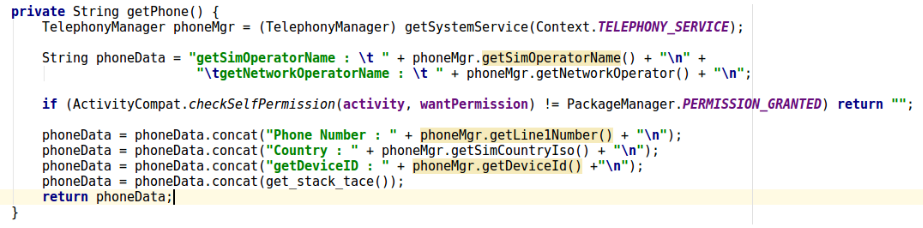
\includegraphics[width=\textwidth]{getPhone_source.png}}
		\caption{Source code of the method getPhone( )}
		\label{fig:getPhone_source}
	\end{figure}
	
	\begin{figure}[H]
		\centering
		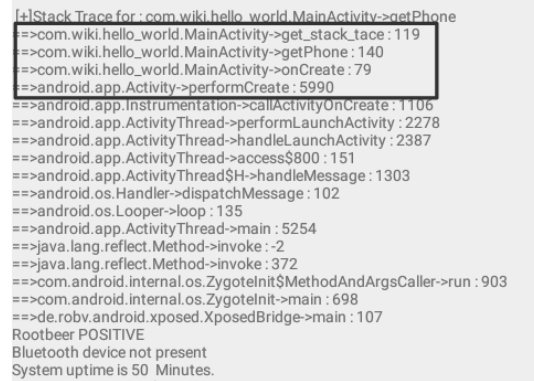
\includegraphics[scale=0.6]{stack_trace_getPhone_unhooked.png}
		\caption{Stack/call trace of the non-hooked method getPhone( )}
		\label{fig:getPhone_trace}
	\end{figure}
	
	
	\paragraph{} Now we will hook this method using frida, below is the procedure:
	\begin{enumerate}
		\item Execute frida-server on guest, if it not running already.
		\item Execute the below python script
		\begin{lstlisting}[language=python]
			import frida, sys, time
			def on_message(message, data):
			if message['type'] == 'send':
			print("[*] {0}".format(message['payload']))
			else:
			print(message)
			jscode = """
			Java.perform(function () {
				// Function to hook is defined here
				var MainActivity= Java.use('com.wiki.hello_world.MainActivity');
				// Whenever button is clicked
				MainActivity.getPhone.implementation = function () {
					// Show a message to know that the function got called
					send('getPhone');
					// Call the original onClick handler
					var output = this.getPhone();
					send(output);
					// Modify return value of getPhone method
					return output+"NNNOOOOTTTT";
				};
			});
			"""
			device = frida.get_usb_device()
			pid = device.spawn(['com.wiki.hello_world'])
			process = device.attach(pid)
			script = process.create_script(jscode)
			script.on('message', on_message)
			print('[*] Running CTF')
			script.load()
			device.resume(pid)
			sys.stdin.read()
		\end{lstlisting}
	\end{enumerate}
	\paragraph{} The above code comprises of two languages, one is the python code that is being executed on the host. Second is the JavaScript code that is injected in the target process. The python script is doing the following:
	\begin{enumerate}
		\item It connects with adb in line "device = frida.get\textunderscore usb\textunderscore device()",
		\item Opens the application process (its paused and need to be resumed)
		\item Attach it to process, adds the JavaScript code store in jscode variable
		\item Registers the callback function to receive messages from guest (send using send("message")
		\item Load the script and resumes the start executing the application opened in 2.
		\item Add stdin to stop application from exiting
	\end{enumerate}	
	In the JavaScript code we are doing following:
	\begin{enumerate}
		\item We open MainActivity using Java.use
		\item We hook the getPhone method, send its original return value and modify the return value.
	\end{enumerate}
	\paragraph{} Figure \ref{fig:hello_world_app_hooked} shows the messages sent by frida-server to host including our messages and confirms that the method getPhone is hooked by sending back the string "getPhone" and return value of this method. We made this output(build info+ stack trace) rather short to be able to show it in on one screen. and figure \ref{fig:hello_world_terminal_hooked} , and modified returned value in app window by appending an easy to spot string of "NNNNNOOOOOOOTTTTT" to the return string of the getPhone and this can be seen in figure \ref{fig:hello_world_app_hooked}. Also notice the extra calls in stack trace and compare it with the previous one in which no hooking was involved.
	
\begin{figure}[H]
	\centering
	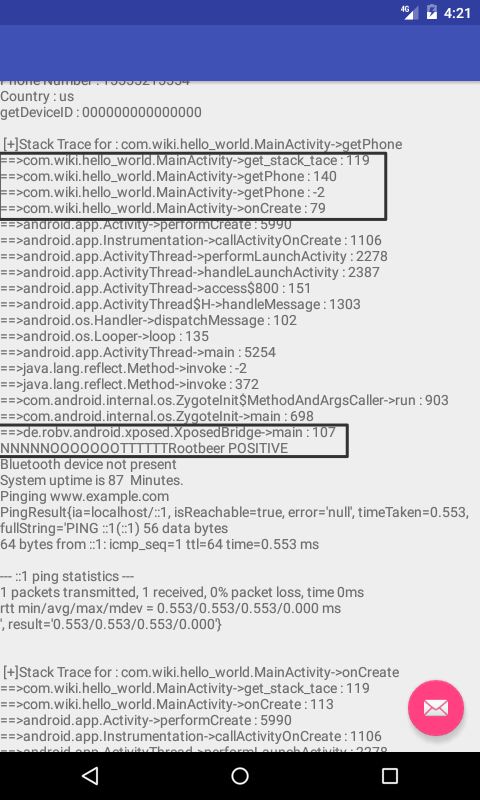
\includegraphics[scale=0.4]{hello_word_after_hooking.png}
	\caption{Hooked output on app screen}
	\label{fig:hello_world_app_hooked}
\end{figure}

\begin{figure}[H]
	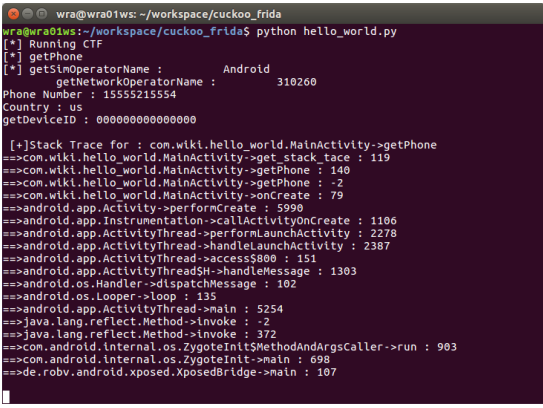
\includegraphics[width=\textwidth]{hello_world_terminal_output.png}
	\caption{terminal output of app with hooked getPhone()}
	\label{fig:hello_world_terminal_hooked}
\end{figure}
	
	
	
	\paragraph{Example 2: Getting Javascript wrapper for Java classes (Logcat example):} In this example we will demonstrate on how to use the Java API of android inside our injected JavaScript code. Frida allows us to get wrappers for Java methods of android and use them inside of our injected code as we wish. Python code for this example is below. In this code it can be seen that we use Java.use method provided by JavaScript API of frida to get a JavaScript wrapper for class 'android.util.Log'. We then check for log.i method and if it is present, we call it.
	\begin{lstlisting}[language=python]
		import frida, sys, time
		def on_message(message, data):
		if message['type'] == 'send':
		print("[*] {0}".format(message['payload']))
		else:
		print(message)
		jscode = """
			Java.perform(function () {
				// Function to hook is defined here
				var MainActivity = Java.use('com.wiki.hello_world.MainActivity');
				var Log = Java.use('android.util.Log');
				if (Log.i){
				send("Sending message");
				Log.i("Xposed_frida", "[+][+] Successful Log message [+][+]");
				}
			});
		"""
		device = frida.get_usb_device()
		pid = device.spawn(['com.wiki.hello_world'])
		process = device.attach(pid)
		script = process.create_script(jscode)
		script.on('message', on_message)
		print('[*] Running CTF')
		script.load()
		device.resume(pid)
		sys.stdin.read()
	\end{lstlisting}
	
	\paragraph{} The result of running this script can be seen in figure \ref{fig:wrapping_logcat}. This example demonstrate the power of frida, we can use all the Java functionality inside our script.
	\begin{figure}[H]
		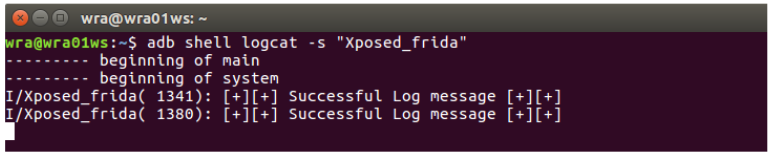
\includegraphics[width=\textwidth]{wrapping_logcat.png}
		\caption{Terminal output }
		\label{fig:wrapping_logcat}
	\end{figure}
	
	
	\paragraph{Example 3: Interactive Frida (Frida-CLI):}
	One can get an interactive frida shell by entering the following command:
	\begin{lstlisting}[language=bash, numbers=none]
		frida -U --no-pause -f com.package.name
	\end{lstlisting}
	This command will launch the app and gives an interactive shell where you can type Javascript to do your stuff. If you want to write your
	script before the app launches, omit the --no-pause parameter. Because of the auto-complete feature as show in figure \ref{fig:interactive_frida} this is a great place to discover methods and features supported by frida.
	\begin{figure}[H]
		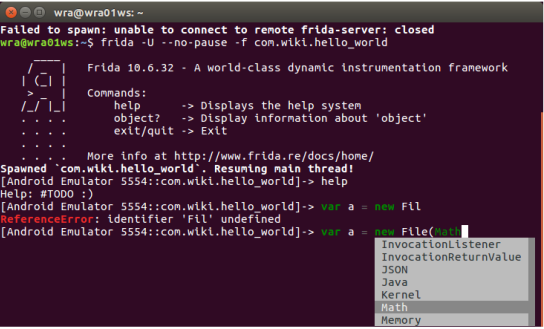
\includegraphics[width=\textwidth]{interactive_frida.png}
		\caption{interactive frida output }
		\label{fig:interactive_frida}
	\end{figure}

	\paragraph{Example 4: Compile a Frida script comprised of one or more Node.js modules (File reading test case):} Its not much useful to code in simple JavaScript in our use case scenario. Our use case scenario is same as server side programming using JavaScript and its important to be able to use NodeJS. Frida provides a tool for that called "Frida-Compile" \cite{frida_compile}. This tool compile a Frida script comprised of one or more Node.js modules. In layman terms, its takes a NodeJS projects and create a single file payload/agent that we can load using the "load\textunderscore script" method that comes with frida.
	\paragraph{} Before using first we need to install frida-compile and it comes a node package and we can use node package manager (npm) to install it. We will install it with -g parameter to make it available globally.
	\begin{lstlisting}[numbers=none]
	$ sudo npm install frida-compile -g
	\end{lstlisting}
	
	
	\paragraph{} To make sure that frida-compile is installed correctly and to see help we will type the following command:
	\begin{lstlisting}
	$ frida-compile --help

	Usage: frida-compile [options] <module>
	
	Options:
	
	-V, --version             output the version number
	-o, --output <file>       set output <file>
	-w, --watch               watch for changes and recompile
	-b, --bytecode            output bytecode
	-x, --no-babelify         skip Babel transforms
	-S, --no-sourcemap        omit sourcemap
	-c, --compress            compress using UglifyJS2
	-a, --use-absolute-paths  use absolute source paths
	-h, --help                output usage information	

	\end{lstlisting}	
	
	\paragraph{} Now the command to compile a NodeJS project/code is below. Here app.js the NodeJS main file and payload.js is the output file that we will load in python binding using load\textunderscore script.
	\begin{lstlisting}
	$ frida-compile app.js -o payload.js
	\end{lstlisting}
	
	Below are scripts that I used to open a text file located on the device and send its content to host. Make sure that you install the required packages frida-fs \cite{frida_fs} using npm. Here is the source code of app.js:
	
	\begin{lstlisting}[language=JavaScript]

		'use strict';		
		const fs = require("frida-fs");
		Java.perform(function () {
			var readStream = fs.createReadStream("/data/local/tmp/hooks.json");
			var text = "";
			readStream
				.on('readable', function () {
					var chunk;
					while (null !== (chunk = readStream.read())) {
						text = text.concat(chunk);
					}
				})
			.on('end', function () {
			send(text);
			});
			});
	\end{lstlisting}

	\paragraph{} In this python code we first compile the NodeJS code using frida-compile and then use the output script as a normal JavaScript payload shown in every other example.
	\begin{lstlisting}
	import frida, sys, time, os, subprocess
	
	def on_message(message, data):
		try:
			if message['type'] == 'send':
				print("[*] {0}".format(message['payload']))
			else:
				print(message)
		except:
			print(message)
		
	frida_ready = False
	device = frida.get_usb_device()
	while not frida_ready:
		try:
			time.sleep(5)
			pid = device.spawn(['com.wiki.hello_world'])
			frida_ready = True
		except Exception as e:
			print("Frida not ready yet " + str(e))
	
	time.sleep(1)
	
	cwd = os.path.dirname(__file__)
	print("Working Directory is : "+ cwd)
	
	print ("Compilation result is: \n")
	print(subprocess.Popen("frida-compile index.js -o compiled.js", shell=True).communicate())
	
	
	try:
		process = device.attach(pid)
		script = process.create_script(
			open("/home/wra/workspace/cuckoodroid/frida-scripts/file_io/compiled.js").read())
		script.on('message', on_message)
		print('[*] Running Frida')
		script.load()
		device.resume(pid) # At end Important, otherwise app will start and you will miss some early code execution as hooks won't be inplace at that time.
	except Exception as e:
		print("Frida python binding code error :" + str(e))
	
	sys.stdin.read(1)
	
	\end{lstlisting}

	\paragraph{} Below the output, you can see that the contents of hooks.json file was sent by guest and we displayed it on host.
	\begin{lstlisting}
	Working Directory is : 
	Compilation result is: 
	
	(None, None)
	[*] Running Frida
	[*] {
	"hookConfigs": [
	{
	"class_name": "android.telephony.TelephonyManager", 
	"method": "getDeviceId", 
	"thisObject": false, 
	"type": "fingerprint" 
	}, 
	{
	"class_name": "android.telephony.TelephonyManager", 
	"method": "getSubscriberId", 
	"thisObject": false, 
	"type": "fingerprint" 
	}
	], 
	"trace": false
	}
	\end{lstlisting}
	
	\section{Chapter conclusion} In this chapter we gave an introduction to Frida. We tried to show how powerful it is by some simple examples. We also concluded that integrating Frida to CuckooDroid can have several benefits and it will help keep the CuckooDroid in supporting higher versions of Android. 

\end{document}